\documentclass[class=article, crop=false]{standalone}


\usepackage{amsfonts}
\usepackage{amsmath}
\usepackage{booktabs}
\usepackage{caption}
\usepackage{import}
\usepackage{multicol}
\usepackage[subpreambles=false]{standalone}
\usepackage{tikz}

\usepackage[linesnumbered,ruled,vlined]{algorithm2e}
\newcommand\commentfont[1]{\footnotesize\ttfamily\textcolor{blue}{#1}}
\SetCommentSty{commentfont}

\usepackage[backend=biber]{biblatex}
\addbibresource{references.bib}

\usepackage{geometry}
\geometry{
   a4paper,
   left=20mm, right=20mm,
   top=20mm, bottom=25mm
}
 
\usepackage{hyperref}
\hypersetup{
  colorlinks=true,
  linkcolor=blue,
  citecolor=black,
}


\begin{document}




\section{Methods}
\label{sec:methods}

\subsection{Data set}The models are trained predominantly on the Headspace dataset \cite{Dai2019}, a set of 3D images of the human head that is available for university-based non-commercial research. The collection consists of 1519 subjects, each wearing tight-fitting latex caps to avoid holes in the mesh on the scalp of the patient. The photos are captured by a 5-camera setup around the head of the person (Fig. \ref{fig:stereophotogrammetry}).
\import{}{import/stereophoto.tex}The images have a high quality, consistent illumination and are pose normalized. 1200 samples include annotations, but as they were automatically generated, the quality of the labels differs for each landmark type and each sample. Nonetheless, due to the sheer number of annotated samples, the Headspace data is used as training data for the first network that extracts rough landmark locations. Manual inspection shows that the Zhu-Ramanan mixture of trees algorithm in subsequent 2D to 3D projection similar mistakes for most samples, e.g. the landmarks are placed a few millimetres too low. %'although often inaccurate predictions, they are consistent (note: move to discussion). error patterns 
In total, the Headspace data set comes with 68 landmarks per image. However, many of them are non-surgical and ill-defined and can be discarded for the purpose of finding landmarks to assist oral and maxillofacial surgery. Out of the 68 landmarks, we keep 12 medically relevant, anatomical landmarks (see table \ref{table:landmark_names}). to properly evaluate the results and to train the refinement network, we manually annotate the 12 landmark positions for around 350 Headspace samples. Although not placed by a specialist, these labels are considerably more accurate, as they are human-annotated instead of to machine-annotated.

Furthermore, 3D photos from Radboudumc are used to validate the method further. The in-house meshes have lower quality, and the illumination varies greatly. The 3D photos are not pose normalized oriented differently in space than the Headspace photos. As the patients do not wear any latex caps, holes and artefacts in the region of the hair are common. Also, most 3D photos are captured by a 2-camera-setup, namely one from the front-left and one from the front-right. Consequently, meshes reconstructed from such photos have big holes in the back of the cranium as they only capture the frontal view.

See figure \ref{fig:data_hs_umc} for a visualization of the photos from the Headspace data set and the Radboudumc data set.
\import{}{import/data_hs_umc.tex}
% As the reconstruction of the mesh for subjects with long hair and hair styles that do not form a flat surface is especially difficult

\subsection{Data Preparation}
The 3D meshes are available as wavefront object’files (OBJ.). This file format contains information about vertices, edges, faces, normal vectors and texture.
Vertices are points in the Cartesian coordinate system defined by x, y and z. Meshes also contain surface data in edges and faces that define the interconnectivity between vertices. Normals define vectors that are perpendicular the to face. Textures add color information by storing uv-coordinates per vertex. The uv-coordinates map the vertex to a bitmap file (.BMP) to refer to the corresponding color  \cite{Jong}.
% texel sampling meshlab pymeshlab
To simplify the problem, the networks process point clouds instead of meshes. Using PyMeshLab, a Python interface for the 3D mesh processing software Meshlab \cite{meshlab}, filters are applied to prepare the point cloud data. Firs,t a point sampling is applied, optionally with corresponding normals and colors. This process preserves the vertices of the mesh while discarding edge and face information. In literature, irregular sampling was identified as a factor that can potentially hamper certain machine learning methods. Thus, we use a sampling technique (‘Texel Sampling’) that was observed to produce evenly distributed points on the surface. Depending on the network the data is prepared for, the point cloud can be simplified to reduce the resolution. The refinement network takes as input the full resolution point cloud. In contrast, the initial network is applied on low-resolution data. Around 30,000 vertices are sampled for the low-resolution point cloud.

The 68 landmarks in the Headspace data are given by a reference to the vertex index in the mesh. The manually annotated landmarks in 3DMedX\footnote{3DMedX is software from Radboudumc that allows 3D reconstruction using DICOM files from (CB)CT-scans or MRI scans and offers tools for the evaluation of orthognathic surgery. It also supports the creation of custom workflows, e.g. for registering landmarks.}\cite{3dmedx} are saved as coordinates in Comma-separated values files. If the point cloud has been sampled before,
the original landmark coordinates do not point to a vertex in the downsampled point cloud anymore and must be re-calculated. The corresponding landmark point for the downsampled mesh is re-calculated by picking the vertex with the smallest distance to the original coordinate. Currently, this is done in a naive way by iterating over each vertex in the mesh. This step can be sped up significantly by applying a more sophisticated algorithm. Constructing the targets as simple point landmarks can have certain disadvantages. For example, the neural network is more difficult on sparse positive cases. Therefore, we construct point clusters around the landmark point to create regions that the network can learn more easily. The point closest to the landmark has the highest activation (1.0), points in the neighborhood are assigned decreasing activations with decreasing proximity and points outside the landmark regions are considered background points with activation of zero. The exact activation scheme differs depending on which network the targets are prepared (see table \ref{tab:activation-scheme} for details). An alternative, perhaps more balanced solution would be to assign activations based on a continuous distribution such as the Gaussian distribution. The approach of generating point clusters around landmarks increases the proportion of points with an activation higher than zero and improves the class imbalance problem.

\begin{table}[]
\centering
\begin{tabular}[t]{lcc}\toprule
 & \multicolumn{2}{c}{Distance range} \\
\cmidrule(lr){2-3}
Activation & Initial & Refinement\\
& network & network\\
\hline
1.0        & closest point  & closest point    \\
0.75       & up to 3.0mm & up to 1.5mm    \\
0.5        & 3.0 to 4.5mm & 1.5 to 3.0mm   \\
0.25       & 4.5 to 6.0mm & 3.0 to 4.5mm  \\
0.0       & higher than 6.0mm & higher than 4.5mm  \\\bottomrule
\end{tabular}
\caption{\textbf{Target activation scheme.} The points are assigned an activation depending on the proximity to the respective landmark.}
\label{tab:activation-scheme}
\end{table}


To build a landmark detector that can discriminate between landmark types and to allow for overlapping activation clusters (meaning one point can be part of the neighborhood of multiple landmarks), each landmark cluster is stored a channel.

However, storing the activation for each point is very memory-consuming. To compress the label files, only the vertex indices and activation for points with an activation higher than zero are explicitly stored. All other points are assumed to have an activation equal to zero. This reduces the necessary information to store from $\textit{total vertices} \times \textit{}{landmarks}$ for the sparse matrix representation to $\textit{vertices in landmark regions} \times \textit{2} \times \textit{landmarks}$ where the factor 2 arises as the compressed representation not only needs to save the activation but also additional vertex index information. The sparse labels are saved as serialized Python object structures, so-called pickle objects.
\import{}{import/gt_hs_clusters.tex}


\subsection{DiffusionNet}
In this work, DiffusionNet \cite{sharp2022diffusionnet} is used to extract surface features from faces. With a diffusion operation, surface information is propagated through space. Diffusion is defined by the heat equation 

\begin{equation}
    \frac{d}{dt}u_t = \Delta u_t,
\end{equation}
where $\Delta$ is the Laplacian and $u_t$ the diffused distribution. The action of diffusion is defined as 

\begin{equation}
    H_t(u_0) = e^{-t\Delta}u_0,
\end{equation}
where the heat operator $H_t$ creates a diffused distribution based on the initial distribution $u_0$. With increasing time, diffusion becomes a global smoothing process, thus approaching the average for $t \to \infty$. An advantage of this technique is that diffusion is fairly robust to how the surface is sampled. In practice, diffusion needs to be discretized by replacing the distributional Laplacian with the weak Laplace matrix $L$, which, together with the mass matrix $M$ (diagonal matrix of areas associated with each vertex) yields the rate of diffusion $M^{-1}Lu$.

A diffusion layer $h_t : \mathbb{R}^P \to \mathbb{R}^P$ creates the diffused matrix for V points and the feature channel $u$. The time $t \in \mathbb{R}_{\geq 0}$ is a learned parameter per feature channel. The time parameter represents the spatial support and is analogous to the receptive field in CNNs, dependent on the filter size and pooling. Since diffusion time is a learned parameter per feature channel, the spatial support is more flexible and does not need to be manually chosen. Interestingly, Sharp et al. give theoretical proof that shows that replacing convolution by diffusion maintains the expressive power of the network.

The evaluation of the diffusion layer $h_t(u)$ needs to be efficient and differentiable to allow network training. Sharp et al. propose to use a direct implicit timestep or spectral expansion. This work uses spectral expansion as the diffusion can be more efficiently computed at evaluation time, with the trade-off that the eigenbases need to be precomputed. Diffusion is truncated to a lower frequency basis $k$, which leads to some approximation error, but no noticeable effect on network performance.

Since diffusion only allows for radially symmetric filters, in addition, spatial gradients are used to enable directional filters. In the case of point cloud input without normals, the normal vectors per point are approximated by the m-nearest neighbors. A least squares approximation then calculates gradient values in the tangent plane which yields the sparse gradient matrix $G \in \mathbb{C}^{PxP}$. Applying the feature vector $u$ to the sparse matrix yields the gradient tangent vector per point.
% Additionally, gradient features
\documentclass[crop=false]{standalone}

\usepackage[subpreambles=false]{standalone}
\usepackage{import}
\usepackage{graphicx}
\usepackage{subcaption}
\usepackage{tikz}

\begin{document}

\begin{figure*}
  \centering
  % \hspace*{-0.08\linewidth}
  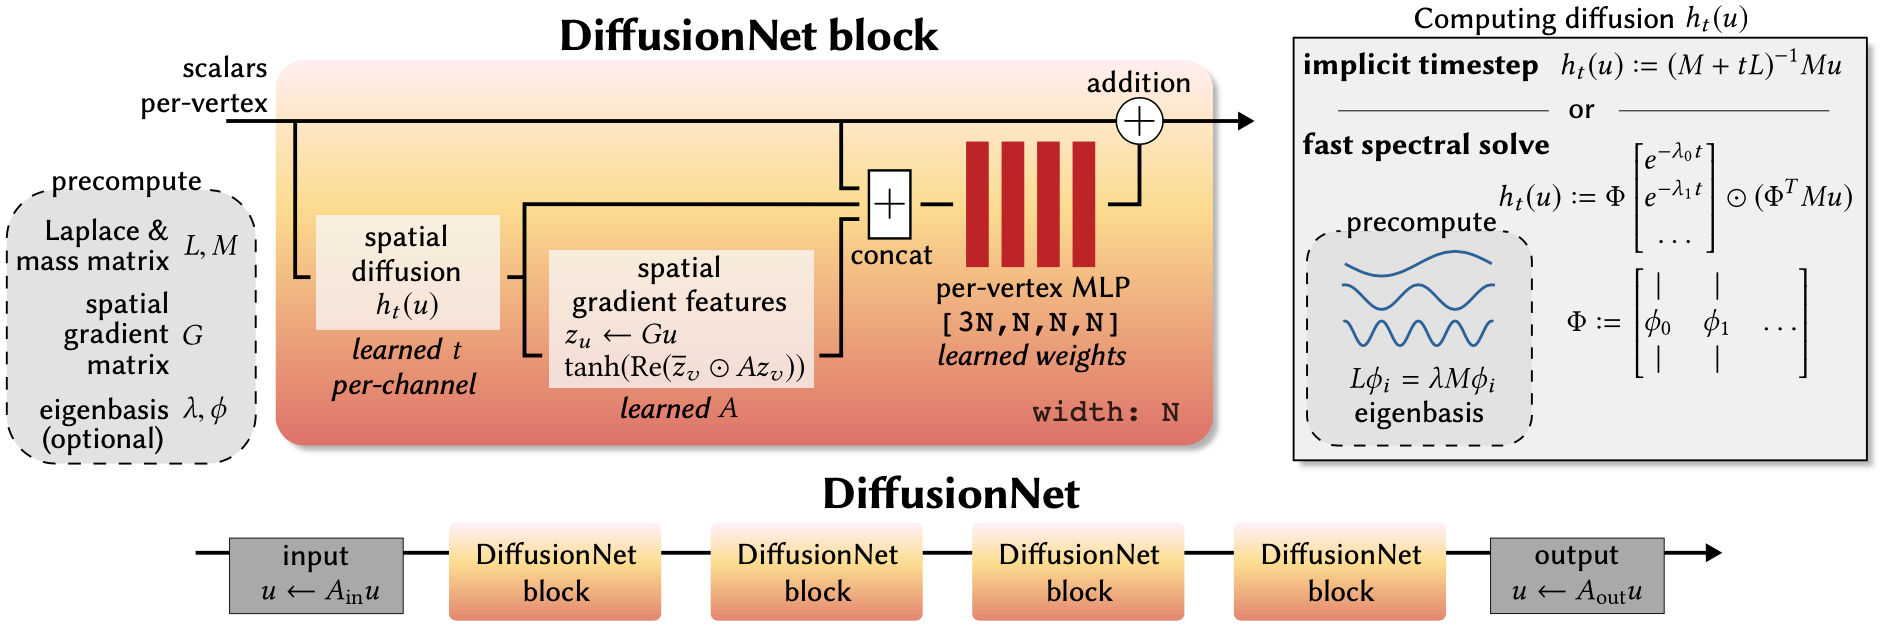
\includegraphics[width=\linewidth]{thesis/methods/import/imgs/diffusionnet_architecture.png}
  %\vspace*{-0.06\linewidth}
  \captionof{figure}{
    \textbf{DiffusionNet architecture.}
    \small After the precomputation of necessary operators, the input is applied to several blocks. In each block, spatial gradients and diffused features are fed into a point-wise MLP with shared weights, and residual connections facilitate training. In this work, diffusion is computed by spectral acceleration. 
  }
  \label{fig:diffusionnet_architecture}
\end{figure*}

\end{document}


% diffusion at various learned timescales fol- lowed by a learned pointwise function 

\subsection{Implementation}
We define a point set \begin{math}X=\{X_i \in \mathbb{R}^F,\hspace{0.3cm}i = 1,2,...,P\}\end{math} as the input of the model, where $P$ defines the number of points in the point cloud, $F$ the dimension, and $x_i$ is the 3D coordinate of each point in the Cartesian reference system. Note that even in a 3-dimensional reference system, $F$ is not restricted to 3 as we can use other point-based features such as the color or the normal vector.

Most machine learning algorithms require a fixed input size. DiffusionNet can deal with a flexible input size, making sampling or simplification for standardizing the number of vertices unnecessary.

The problem is approached as a point-wise regression problem as opposed to directly regressing coordinates (see appendix \ref{sec:coord_reg_vs_pw_reg} for details).

The network and data loading is implemented in PyTorch \cite{NEURIPS2019_9015}, a popular deep learning library that supports GPU acceleration.

DiffusionNet requires precomputing the Laplacian, mass matrix and gradients for spectral acceleration and saving them in a cache to quickly access them during data loading to avoid repeating the computationally expensive operations. Together with these operators we additionally cache the labels. Since the labels were previously compressed to reduce disk space, they are decompressed as the sparse representation is needed for training.

As DiffusionNet is originally built for classification, segmentation and functional correspondence tasks. We adapt the network architecture to output per-point scores for each landmark channel by changing the size of the last layer to $\textit{vertices} \times \textit{landmarks}$.


\subsection{Training}
The networks are trained with the weighted mean squared error (WMSE) metric. Mean squared error (MSE) guarantees the error to be strictly positive the square punishes very large differences:
\begin{equation}
    MSE = \frac{1}{n}\sum^n_{i=1} (Y_i - \hat{Y}_i)^2
\end{equation}
Even with modelling landmark regions, activations $> 0$ are rare due to an imbalance between background and landmark regions. We introduce weights to counteract the class imbalance problem. Points with higher activations are assigned higher weights and background points are assigned a weight of one. The exact weighting scheme differs for the initial network and the refinement network, because they exhibit different imbalances between background and landmark regions. The weighting schemes ensure that the network pays sufficient attention to finding points in landmark regions while not overemphasizing on them, which can lead to exceedingly large and blurry clusters.

\subsection{Initial Network}\import{}{import/pred_hs_clusters.tex}The initial network takes as input the full point cloud which typically involves the cranium, neck and possibly some artefacts and other body parts of the upper body depending on the photo and mesh reconstruction. The original meshes can have 100,000 to 200,000 vertices. Processing the photos in full resolution would lead to excessively high memory footprints and very long times for the precomputation of the operators. Thus, around 30,000 vertices are sampled and used as input for the initial network (see figure \ref{fig:gt_hs_clusters}). Due to the big class imbalance, the weighting scheme is set quite aggressively (see table \ref{tab:weighting-scheme})
\begin{table}[]
\centering
\begin{tabular}[t]{lll}\toprule
 & \multicolumn{2}{c}{Weight} \\
\cmidrule(lr){2-3}
Activation & Initial & Refinement\\
& network & network\\
\hline
0.0        & 1  & 1    \\
0.25       & 25 & 5    \\
0.5        & 50 & 10    \\
0.75       & 75 & 15    \\
1.0        & 100 & 20  \\ \bottomrule
\end{tabular}
\caption{\textbf{Weighting scheme.} The initial network uses more aggressive weighting for higher activations to combat class imbalance. For the refined network smaller weights are sufficient because of less prominent class imbalance.}
\label{tab:weighting-scheme}
\end{table}

\subsection{Refinement Network}
The refinement network is applied to regions around landmarks. The regions are sampled in full resolution to enable a higher potential accuracy. For training, a sphere around the ground truth landmark with a radius of 2.5cm is cut out. To prevent the model from overfitting by consistently selecting the center point of the sphere as the mid point of the predicted cluster, a random translation of up to 3mm in each direction is applied. To emphasize the network's focus on the local neighborhood we adapt a more local activation scheme for the targets.

The regional point clouds only comprise around 1000 to 2000 points for the Headspace data, depending on the landmark type. For the Radboudumc data, this number is even lower since the meshes have a lower resolution. This, combined with the chosen activation scheme, leads to a less prominent class imbalance, reflected in the chosen weights.

Similarly, during prediction, a sphere of the same size is cut around the predicted landmark and sampled in high-resolution.


\subsection{Shape Variants}
3D shapes can come in different variants that the network should be invariant to, such as different orientations or different discretization. Varying camera setups or differing preprocessing can lead to different head orientations in space. The network should give the same result regardless of head rotations. The perhaps most straightforward approach is to perform data augmentation. While it can make the network more robust to the presented augmented variants, data augmentation does not scale well as it is not feasible to sample all variations. Additionally, including slightly varied samples in training quickly increases training times. The preferred approach to dealing with shape variants is to design an inherently invariant network to rotations. There is still ongoing research on how to design such invariant networks most efficiently. 

Another way is to use input features that are intrinsically invariant to isometric transformations, thus also to rigid deformations such as rotation. To this end, we include the Heat Kernel Signature (HKS) in our experiments and compare HKS features to raw XYZ coordinate features.

Simple preprocessing steps can already create robustness to scaling and translation. Thus, we center and unit scale the objects. Centering mitigates translations in the x-, y- or z-axis by centering around the average of the point positions. Unit scaling can avoid large variances in head sizes. It should be noted, however, that both centering and unit scaling are applied to the entire point cloud. Because the photos vary a lot in artefacts and different body parts captured, the scaling and centering of the face itself are noisy.

While centering the object is likely unnecessary for the network with HKS features as input, as the features are already invariant to rigid deformations, it can improve robustness for networks with raw coordinate input which is sensitive to translation.
\end{document}
